% Following magic comments allow for compilation of root file
% !TEX root = ../../../../temp_manuscript.tex

\chapter{Introduction}\label{chap:introduction}


Cardiovascular diseases and \gls{COPD} are among the major leading causes of death globally \cite{ritchie2018causes}. Patients with \gls{COPD} are at increased risk of cardiovascular disease\cite{roversi2016chronic, ruparel2019evaluation} and the prognosis in \gls{COPD} is greatly affected by the presence of cardiovascular disease \cite{andre2019COPD, carter2019association}. Non-invasive imaging techniques such as \gls{CT}, together with quantitative image analysis play an increasingly important role in investigating the clinical and pre-clinical stage of cardiovascular disease. \gls{CT} scans are used for lung cancer screening \cite{pedersen2009danish, labaki2017role, mets2012quantitative, wells2012pulmonary, mets2011identification, mets2012computed, singhvi2020computed, heuvelmans2019screening, li2019importance, suh2020coronary,ruparel2019evaluation,oudkerk2017european} where both the heart and the lungs can be assessed in a single, rapid diagnostic test. Therefore in such scans it might be possible to identify both cardiovascular disease and \gls{COPD}.

The aorta and the pulmonary artery are the two largest arteries in the chest. Changes in the shape and the size of the aorta and the pulmonary artery are associated with several cardiovascular diseases including pulmonary hypertension \cite{raymond2014significance, truong2018four}, aortic dilatation and aortic aneurysm \cite{american20102010,wolak2008aortic}, and coarctation of the aorta \cite{frandsen2018ascending, von2002predictors}. The ratio of the diameter of the pulmonary artery to the diameter of the ascending aorta (PA:AA) at the level of pulmonary artery bifurcation is shown to be associated with increased risk of severe exacerbations \cite{rho2018ct,wells2012pulmonary}, and increased mortality \cite{terzikhan2017pulmonary} in patients with COPD. The imaging-based assessment of the shape and size of these arteries for investigating the presence of cardiovascular disease and/or predicting complications in patients with COPD have therefore rapidly gained interest.

To assess abnormalities in the shape and the size of these arteries, diameter measurements are required where measurements derived from 3D segmentations are most reliable. However, performing such measurements manually is labor-intensive and time-consuming. Therefore full automated 3D segmentation and subsequent diameter analysis are desirable.

The focus of this thesis is on automated image analysis for characterization of the shape and diameters of the aorta and pulmonary artery, to facilitate clinical and epidemiological research, assist in early stage diagnosis of aortic aneurysm, and to extract risk factors for the exacerbation of COPD. This Chapter provides a background on the anatomy of the aorta (\cref{sec:AA_Anatomy} and pulmonary artery(\cref{sec:PA_Anatomy}), disease associated with these vessels (\cref{sec:Disease}), theoretic imaging modalities (\cref{sec:Modality} ), image processing challenges (\cref{sec:challenges}),  vascular segmentation (\cref{sec:Segmentation}), followed by contributions and outline of this thesis (\cref{sec:Goals}).
%theoretic imaging and screening
%The focus of this thesis is on automated image analysis for characterization of the shape and diameters of the aorta and pulmonary artery, to assist in early stage diagnosis of aortic aneurysm and to extract risk factors for the exacerbation of \gls{COPD}.
%
%This introduction provides a background on the anatomy of the aorta (Section \ref{AA_Anatomy} and pulmonary artery(Section \ref{PA_Anatomy}), deasease associated with these vessels (Section \ref{Disease}), theoretic imaging and screening (Section \ref{Modality} ), image processing challenges (section \ref{challenges}),  vascular segmentation (Section \ref{Segmentation}), followed by goals and an outline of the remainder of the thesis (Section \ref{Goals}).
%

%################################################################

%\section{Motivation}
%
%%Noncommunicable diseases are diseases of long duration and generally slow progression. In the main types of noncommunicable diseases cardiovascular diseases are the major leading cause of death worldwide followed by cancers and respiratory diseases including chronic obstructive pulmonary disease (\gls{COPD}) as the third biggest cause of morbidity and mortality globaly\cite{owidcausesofdeath2018}.
%Cardiovascular diseases and chronic obstructive pulmonary disease (\gls{COPD}) are the major leading cause of morbidity and mortality globaly\cite{owidcausesofdeath2018}. 
%Non-invasive imaging techniques such as CT, play an increasingly important role in staging the clinical and preclinical stage of the disease.
%
%Cardiovascular diseases are a group of disorders of the heart and blood vessels, where aortic aneurysm is one of the bigest subtypes of it \cite{Roth2017}. Most patients with aortic aneurysm are asymptomatic, not detectable on physical examination, and silent until discovered during imaging examinations performed
%for other purposes like \gls{COPD} or lung cancer screening or other reasons. Detecting aortic dilatation at an early stage enables preventive surgery, which might save lives.
%
%\gls{COPD} is a lung disease characterized by chronic obstruction of lung airflow, associated with typical risk factors—most notably cigarette smoke and is highly prevalent in the ageing population\cite{https://www.who.int/respiratory/\gls{COPD}/definition/en/}.
%Patients with \gls{COPD} are at increased risk of cardiovascular disease\cite{Roversi2016},therefore, it is valuable to analyse the  vessels associated with these both desease types jointly. 
%
%The shape and the diameter of the two large vessels in the body, the aorta and pulmonary artery, are asociated with both cardiovascular diseases and \gls{COPD}, such as aortic aneurysm \cite{Wolak2008d}, coarctation of the aorta\cite{Frandsen2018b}, pulmonary hypertension\cite{Raymond2014a,Truong2018a} and Interstitial Lung Disease\cite{Chin2018a}.
%Furthermore, the ratio of the diameter of the main pulmonary artery  to the diameter of ascending aorta at the level of the pulmonary artery biforcation is shown to be associated with the presence of pulmonary arterial hypertension\cite{Truong2018a} and is a strong predictor for exacerbation in patients with \gls{COPD}\cite{Terzikhan2017a, Rho2018} and Concomitant
%Bronchiectasis\cite{Dou2018a}.
%
%Therefore, it is essentioal to perform such measurements both in large-scale imaging studies and in clinical practice. Manually segmenting these anatomical structures is ,however, very labor intensive, therefore, accurate and reproducible automatic segmentation is necessary.
%
%In this Thesis we focus on automated image analysis for charactrization of the vessel shape and diameter, to help for early stage diagnosis of aortic anuyresum and to predic the exacurbation of \gls{COPD}. This introduction provides a background on the aorta and pulmonary attery(Section .....), theoratic imaging and screening (Section.... ), image processing for vascular segmentation(Section ...), followed by an outline of the remainder of the thisis (Section ....).
 
% In this thesis we  automaticly analyse the theoratic CT scans to segment and  method to segment the aorta and pulmonary artey and to measure the diameters
%
%In this thesis we automaticaly segment the aorta and pulmonary artery and obtain highly accurate measurements of vessel radii.
%
%The shape and the diameter of the two large vessels in body, aorta and pulmonary artery, are asociated with both cardiovascular diseases and \gls{COPD}. In Cardiovascular disease the diameter and shape of the aorta is associated with aortic aneurysm \cite{Wolak2008d} and coarctation of the aorta\cite{Frandsen2018b}. In \gls{COPD} the diameter of the pulmonary artery is associated with pulmonary hypertension\cite{Raymond2014a,Truong2018a} and it has a diagnostic value in patients with Interstitial Lung Disease\cite{Chin2018a}.
%Furthermore, the ratio of the main pulmonary artery diameter to the ascending aorta diameter at the level of the pulmonary artery biforcation is shown to be associated with the presence of pulmonary arterial hypertension\cite{Truong2018a} and is a strong predictor for exacerbation in patients with \gls{COPD}\cite{Terzikhan2017a, Rho2018} and Concomitant
%Bronchiectasis\cite{Dou2018a}.
%
%
%
% Therfore CT images performed for \gls{COPD} screening provide the ability to detect cardiovascular desease such as aortic anerysem in early stages.
%
%
%Lung cancer is the leading cause of cancer death in the United States, and an
%estimated 1.5 million new cases are expected to be diagnosed worldwide in 2010 [9].
%Early detection of lung cancer has been shown to reduce lung cancer mortality [7,
%4], prompting the creation of large clinical trials of lung cancer screening using
%low-dose CT imaging [5]. Small malignant pulmonary nodules can be detected in
%low-dose CT images before they become large enough to cause symptoms, allowing
%for earlier treatment and improved clinical outcomes [7].
%
%Segmentation of the pulmonary arteries also provides a first step toward obtaining highly accurate measurements of vessel radii. Patients with pulmonary
%arterial hypertension (PAH) have been shown to present with enlarged pulmonary
%arteries, as measured by manual observation of CT images [22, 17]. These enlarged
%vessels are at increased risk for fatal dissection and require immediate surgical intervention where possible. Automated segmentation and measurement methods
%have the potential to better quantify vessel enlargement in patients with PAH,
%providing an earlier and non-invasive means of diagnosis [14]

\section{Anatomy} \label{sec:Anatomy}
The aorta and pulmonary artery are the two major arteries in the human body that carry blood away from the heart. The aorta is the biggest artery in the body and is responsible for transporting oxygenated blood from the left ventricle of the heart to the rest of the body. Pulmonary artery is responsible for carrying the deoxygenated or unaerated blood from the right ventricle of the heart to the lungs for oxygenation.

The aorta begins at the bulb-shaped root originating from the left ventricle at the level of the aortic valve and then courses through the chest and abdomen in a candy cane–shaped configuration (Fig \ref{fig:anatomy}). The thoracic aorta is part of the aorta located in the chest (thorax) and includes the aortic root, ascending aorta, aortic arch, and descending aorta. The part of the aorta that passes through the diaphragm is called the abdominal aorta.

The aorta has normally a diameter of aproximately 2 cm. It has a slightly larger diameter at the aortic root and then it narrows progressively as it descends into the abdomen. The aortic root consists of three sinuses of Valsalva, also known as aortic sinuses, which give rise to coronary arteries. The junction of the aortic root to the tubular part of the ascending aorta is called the sinutubular junction. From the sinutubular junction the ascending aorta arises, where from the left side it is adjacent to the pulmonary artery trunk, and arches back over the right pulmonary artery to the posterior part of the chest and becomes the aortic arch. Normally three major branches arise from the aortic arch, the brachiocephalic artery, the left common carotid artery, and the left subclavian artery. These vessels supply blood to the upper body. The descending aorta extends from the aortic arch and descends downwards towards the diaphragm. Behind the descending thoracic aorta is the vertebral column.


The pulmonary artery consists of the trunk, left, and right pulmonary arteries which are relatively large arteries. The pulmonary trunk or the main pulmonary artery, has normally a diameter of aproximately 2-3 cm and is approximately 5 centimeters long. The pulmonary trunk originates from the bottom of the right ventricle of the heart and ascends towards the aortic arch where it is adjacent to the ascending aorta. Below the aortic arch, the pulmonary trunk bifurcates in a "Y" shape into the left and right pulmonary arteries, each of which directs the blood to the corresponding lung. This main branching (pulmonary bifurcation) is located above the heart to the left of the ascending aorta. Both left and right pulmonary arteries divide into smaller branches after they enter the lungs. In this thesis we will only consider the left and right pulmonary arteries before their secondary bifurcation.


A depiction of the Aorta and pulmonary artery anatomy and an axial slice from a CT scan is shown in Figure 1\ref{fig:anatomy}. The aorta has almost a circular shape in an axial plane and the pulmonary artery generally has an round-elliptic shape.

Aorta and pulmonary are surrounded by  ....


%%\section{Anatomy of the Aorta } \label{sec:AA_Anatomy}
%%The aorta is the biggest artery in the human body and is responsible for transporting oxygenated blood from the heart to the rest of the body. The aorta begins at the bulb-shaped root originating from the heart at the level of the aortic valve and then courses through the chest and abdomen in a candy cane–shaped configuration. The thoracic aorta is part of the aorta located in the chest (thorax) and includes the aortic root, ascending aorta, aortic arch, and descending aorta. The part of the aorta that goes through abdomen is called the abdominal aorta.
%%
%%
%%
%%%and descending aorta before it crosses the level of the diaphragm where it becomes the abdominal aorta.
%%% The thoracic aorta supplies oxygenated blood to multiple structures, including the head, neck, upper extremities, and thoracic structures.
%%  
%%The aortic root has a slightly larger diameter and consists of three sinuses of Valsalva. The junction of the aortic root to the tubular part of the ascending aorta is called the sinutubular junction. Aorta at this region is adjacent to the pulmonary artery trunk. From the sinutubular junction the ascending aorta arises and arches back over the right pulmonary artery to the posterior part of the chest and become the aortic arch. Normally three major branches arise from the aortic arch, supplying blood to the upper body. The descending aorta extends from the aortic arch and descends downwards into the body and towards the diaphragm.
%%
%%The aorta has almost a circular shape in an axial plan and the pulmonary artery generally has an round-elliptic shape.
%%
%%
%%
%%\section{Anatomy of the Pulmonary Artery } \label{sec:PA_Anatomy}
%%Pulmonary artery is responsible for carrying the deoxygenated or unaerated blood from the heart to the lungs for purification. The pulmonary artery consists of the trunk, left, and right pulmonary arteries which are relatively large arteries. The pulmonary trunk or the main pulmonary artery is a relatively short and wide artery. It originates from the bottom of the right ventricle of the heart and ascends towards the aortic arch where it is  adjacent to the aortic root.
%%
%%Below the aortic arch, the pulmonary trunk bifurcates in a "Y" shape into the left and right pulmonary arteries, each of which directs the blood to the corresponding lung. This main branching is located above the heart to the left of the ascending aorta. Both left and right pulmonary arteries divide into smaller branches after they enter the lungs. In this thesis we will only consider the left and right pulmonary arteries before their secondary bifurcation.
%%
%%A depiction of the Aorta and pulmonary artery anatomy and an axil slice from a CT scan is shown in Figure 1
%%
%%%The aorta begins at the root, starting from the aortic valve (annulus) and becoming slightly wider in diameter (sinuses of Valsalva), and ends at the beginning of the ascending aorta (sinotubular junction). Ascending aorta ascends upward from the aortic root to the point where the innominate artery branches off the aorta, and the aorta begins to form an arch. Due to little support from surrounding tissue and handling the complete output volume of the cardia, it is considered the most vulnerable part of the aorta. Aortic arch is the curved section of the aorta. Descending aorta begins from the arch and descends downwards into the body and ends at diaphragm.% 

\section{Disease associated with the Shape and the Size of the Aorta and Pulmonary Artery} \label{sec:Disease} % shape of the vessels}
Chronic Obstructive Pulmonary Disease (COPD) is a group of lung diseases characterized by chronic airflow obstruction due to airway inflammation. Cardiovascular disease is a general term for conditions affecting the heart or blood vessels. \gls{COPD} and cardiovascular disease frequently occur together and their coexistence is associated with worse outcomes than either condition alone \autocite{rabe2018cardiovascular}. The aorta and the pulmonary artery are the two largest theoretic arteries where the shape and the size of these arteries are associated with several cardiovascular disease and with the risk of exacerbations and death in patients with \gls{COPD}. 

Changes in the shape and the size of the aorta may indicate aortic dilatation and aortic aneurysm \autocite{american20102010,wolak2008aortic}, and coarctation of the aorta \autocite{von2002predictors}. Aortic aneurysm is a permanent localized abnormal enlargement or bulging of the aorta, having at least a 50$\%$ increase in diameter compared with the expected normal diameter of the artery in question \autocite{american20102010}. In patients with aortic aneurysms, the aortic size has a profound impact on the risk of dissection \cite{davies2006novel, kim2015risk}.  Most patients with a dilated aorta or aortic aneurysm are asymptomatic and difficult to detect on a physical examination. The diagnosis usually is made as during screening in the context of a positive family history or by coincidence on imaging examinations performed for other purposes like lung cancer screening, or when a complication occurs, such as aortic dissection or rupture \autocite{melvinsdottir2016incidence}. In these patients the aortic dissection is often the first presentation and results in death. Aortic aneurysm is one of the cardiovascular diseases observed in patients with \gls{COPD} with smoking as a common risk factor.

Narrowing or constriction of the aorta, typically the descending aorta, is called coarctation of the aorta. Coarctation of the aorta is a common congenital anomaly where long term complications such as aortic aneurysms formation can develop from untreated or treated coarctation\autocite{frandsen2018ascending,von2002predictors}. Since aortic aneurysm associated with coarctation in adults could remain asymptomatic for a prolonged time, aortic aneurysm and dissection are the most common cause of death in patients with coarctation \autocite{teimouri2013congenital}.

Due to this silent process with high risks associaed with aortic aneurysm, detecting the aortic dilation at an early stage is therefore desiered. Accurate assessment of the aortic diameter is a key component in detection of aortic aneurysm and in guiding therapeutic decisions which the risk of dissection, rupture, and death is estimated \autocite{wolak2008aortic}. Aortic diameter is a major criterion for recommending elective operation where detecting aortic dilatation at an early stage enables preventive surgery, which might save lives.


Dilation of the main pulmonary artery is associated with pulmonary aneurysm \autocite{gupta2020pulmonary, park2018pulmonary} and is an important metric for the presence of Pulmonary Hypertension \autocite{raymond2014significance,truong2018four,aluja2018approach}. The dilation and aneurysm in the pulmonary artery is a rare abnormality with life-threatening complications such as pulmonary artery dissection. Similar to aortic aneurysm, pulmonary artery aneurysm can frequently be asymptomatic and are incidentally diagnosed on imaging performed for other reasons \autocite{gupta2020pulmonary}. 
Pulmonary hypertension represents a chronic condition characterized by the increased blood pressure in the pulmonary circulation which can cause structural problems like aneurysm of dissection of pulmonary arteries. The location and the size of the enlargement in the diameter of pulmonary artery on CT play an important role in diagnosis and guide the clinician in management of Pulmonary Hypertension \autocite{aluja2018approach}. Dilatation of the main pulmonary artery or major branch vessels has been identified as markers of the presence of Pulmonary Hypertension and is often the first imaging finding to suggest the diagnosis. Enlarged vessels are at increased risk for fatal dissection and require immediate surgical intervention where possible.

Moreover the ratio of the diameter of the pulmonary artery to the diameter of the ascending aorta at the level of pulmonary artery bifurcation (PA:AA) is associated with the presence of pulmonary hypertension \autocite{truong2018four} and is shown to be a strong predictor for exacerbation \autocite{wells2012pulmonary,rho2018ct} , and increased mortality \autocite{terzikhan2017pulmonary} in patients with \gls{COPD}.
 

Figure felan shows 4 different disease with the changes in the shape of the aorta and PA.:


%Changes in the aorta and the pulmonary aretery may indicate cardiovascular diseases including pulmonary hypertension [4, 5], aortic dilatation and aortic aneurysm [6], and coarctation of the aorta [7]. The ratio of the diameter of the pulmonary artery to the diameter of the ascending aorta (PA:AA) at the level of pulmonary artery bifurcation is shown to be associated with the presence of pulmonary arterial hypertension [5] and is associated with poorer health status [8], increased risk of severe exacerbations [9, 10], and increased mortality [11] in patients with \gls{COPD}.

%
%Abnormality in the shape of the aorta \cite{Goldstein2015} casues diseas such as coarctation of the aorta\cite{Frandsen2018}, which is a narrowing or constriction in a portion of the aorta and aortic aneurysm\cite{Wolak2008}, which is an enlargement of the aorta in a balloon-like bulge that can dissect or rupture.

%Aortic aneurysm with the risk of acute dissection is an important cause of mortality in the western world\cite{Roth2017}. Most patients with a dilated aorta or aortic aneurysm are asymptomatic. The diagnosis can be made as during screening in the context of a positive family history or by coincidence on imaging examinations performed for other purposes like lung cancer screening\cite{Mets2012}. In patients with aortic aneurysms, the aortic size has a profound impact on the risk of dissection \cite{Davies2006a, Kim2015a}. Detecting aortic dilatation at an early stage enables preventive surgery, which might save lives.

%Dilation of the main pulmonary artery is associated with pulmonary artery aneurysm\cite{Park2018} and is an important metric for pulmonary hypertension \cite{Raymond2014,Truong2018}. 
%
%The ratio of the dimaeter of the pulmonary artery to the diameter of the aorta at the level of pulmonary artery bifurcation is shown to be a strong predictor for exacerbation in patients with \gls{COPD}\cite{terzikhan2016,rho2018} and Concomitant Bronchiectasis\cite{Dou2018} and is associated with the presence of pulmonary hypertension\cite{Truong2018}.


%Also the pulmonary arterial pressure elevation leads to pulmonary arterial dilation, which is not independently influenced by the presence or severity of Interstitial Lung Disease, therefore the pulmonary artery diameter has diagnostic value in patients with and without Interstitial Lung Disease\cite{Chin2018}. 
%

\section{Theoretic Imaging Modality}  \label{sec:Modality} 
\section{Theoretic Imaging Modalities}
Medical imaging plays a significant role in disease prevention, early detection, diagnosis, and treatment. Computed tomography (CT) and magnetic response imaging (MRI) are the common noninvasive imaging modalities used to visualize the cardiac structures. 

CT is a projection-based imaging modality that uses tomographic reconstruction of x-rays to generate cross-sectional images of the body. In CT, cross-sectional images generated from the combination of multiple X-ray projections acquired at many different orientations around the body, are reconstructed into a 3D image volume. Based on the attenuation of X-rays in various tissue types, CT provides detailed images and an accurate density of any part of the body, including the bones, muscles, fat, organs, and blood vessels. These densities are expressed using the Hounsfield Unities (HU), with water having a value of zero HU. Tissues with higher density than water such as bone have positive HU and are visualized in brighter colors, while structures with less density than water such as air appear darker with negative HU. Currently, with the use of multi-detector and multi-source CT the temporal and special resolution of CT imaging has increased.\autocite{raman2013ct}. 

Contrast-enhanced \gls{CTA}, improves the contrast and the resolution of the vasculature by the administration of iodinated contrast media. 
However, beside the disadvantage of using ionizing radiation in \gls{CT}/\gls{CTA}, though rare, the contrast agent can also produce undesired side effects such as allergic reactions and kidney damage. 
Therefore, current improvements in CT imaging and image analysis are often aimed at significant dose-reduction for providing a safer imaging procedure\autocite{raman2013dosereduction}. Lowering the dose leads to reduction of the image quality and resolution while introduces higher noise level. Low-dose non-contrast CT provides an acceptable image quality with a lower risk of exposure to ionizing radiation, less side effects and subsequently lower procedural costs. A axial plane of a CTA and a low-dose non-contrast CT is shown at Figure \cref{fig:CT_CTA}. It can be clearly seen that in CTA scan, the anatomical structures are clearly defined and delineated, whereas in the non-contrast CT, with the presence of noise there is an unclear border between the vessel borders and the surrounding structures.

\begin{figure}[hbt]
    \centering
    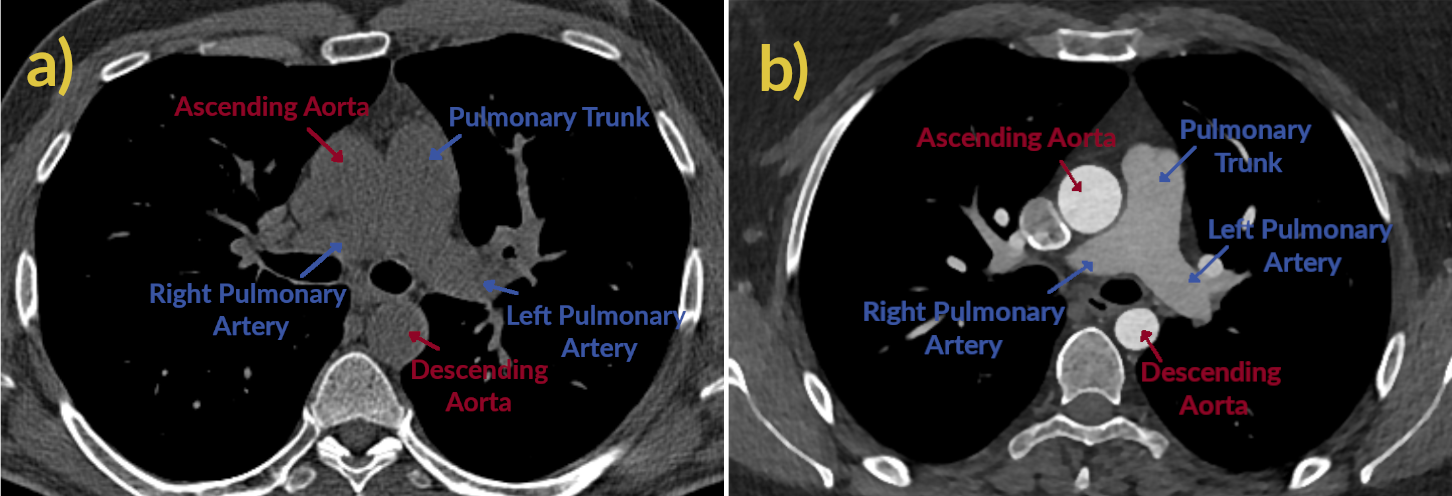
\includegraphics[width=1\textwidth]{Figures/Scans_CT_CTA.png}
    \caption{(a) Axial plan of a low-dose non-ECG-gated, non-contrast CT scan where the boundaries between the arteries are blurred and unclear with a high noise level. (b) Axial plan of a CTA scan where the boundary of the arteries are clearly visible and distinguishable.}\label{fig:CT_CTA}
\end{figure} 


MRI is an imaging modality that utilizes the principle of strong magnetic fields and radiofrequency waves to construct detailed 3D image volumes of the body. Unlike CT, MRI provides a better soft tissue contrast, but it has a lower in-plane spacial resolution and is a more expensive modality. 

Even though MRI has no risk of ionizing radiation, \gls{CT} is generally preferred and widely used in clinical practice for its faster acquisition time, better isotropic spatial resolution, convenience, and easier access. Chest CT often is the imaging modality of choice for diagnosis and follow-up of patients with aortic pathology and is the reference image modality for the study of lung disease and pulmonary vasculature. Many patients with and at risk for \gls{COPD} undergo a low-dose non-contrast thoracic CT for lung cancer screening. With the growing use and widespread availability of low-dose non-contrast thoracic CT scans for lung cancer screening \autocite{pedersen2009danish, oudkerk2017european}, there is an opportunity to measure the aorta and pulmonary arteries in these scans in order to investigate the presence of early-stage cardiovascular disease and/or predict complications in patients with \gls{COPD}.


%CT is a noninvasive imaging modality that allows reconstructing cross-sections of the patient’s body into a 3D image volume. CT generates cross-sections of the body by combining multiple X-ray projections acquired at many different orientations around the patient. recunstructs images based on the difference in the attenuation of X-rays by the varius tissuue types.


%CT is a projection-based imaging modality that creates 3D image volumes using tomographic reconstruction of x-ray.
%Ct is a noninvasive imaging modality that creates 3D image volumes based on the 

%lowering the dose leads to reduction of the image quality 


%CT is a noninvasive imaging modality that recunstructs images based on the difference in the attenuation of X-rays by the varius tissuue types.CT provides detailed images of any part of the body, including the bones, muscles, fat, organs, and blood vessels. In CT high density structures such as bone have high attenuation value (250 to 1000 Hounsfield Units(HU)) and are visualized in white, while less dense structures such as fat and vasculature appear darker with lower HU where air with the lowest attenuation value ($−600$ to $−1000$ HU) is visualized in black. Contrast-enhanced CT angiography (CTA), improves the contrast and the resolution of the vasculature by the administration of iodinated contrast media. Low-dose non-contrast CT without the full radiation exposure inherent in standard CT protocols, has a lower risk of exposure to ionizing radiation and subsequently lower procedural costs. 



%and CT is a noninvasive imaging modality that uses x-rays to provide detailed images of any part of the body, including the bones, muscles, fat, organs, and blood vessels are visualized. Contrast-enhanced CT angiogram (CTA) provides enhanced resolution and contrast by the administration of iodinated contrast media. Non-contrast CT with no injected contrast has a lower risk of exposure to ionizing radiation and lower procedural costs. Compared to CTA and non-contrast CT, low-dose non-contrast CT has a lower resolution and higher noise level, however, it provides accurate anatomical information without the full radiation exposure inherent in standard CT protocols. Figure .... shows a CTA scan and a low-dose non-contrast CT scan. It can be clearly seen that in CTA, the anatomical structures are clearly defined and delineated, whereas in the non-contrast CT, with the presence of noise there is an unclear border between the vessel borders and the surrounding structures\autocite{Labaki2017}.
%
%Although MRI has no risk of radiation, CT is generally preferred and widely used in clinical practice for its faster acquisition time, better isotropic spatial resolution, convenience, and easier access. Chest CT often is the imaging modality of choice for diagnosis and follow-up of patients with aortic pathology and is the reference image modality for the study of lung disease and pulmonary vasculature. Many patients with and at risk for \gls{COPD} undergo a low-dose non-contrast thoracic CT for lung cancer screening.
%
%With the growing use and widespread availability of low-dose non-contrast thoracic CT scans for lung cancer screening \autocite{pedersen2009danish, oudkerk2017european}, there is an opportunity to measure the aorta and pulmonary arteries in these scans in order to investigate the presence of early-stage cardiovascular disease and/or predict complications in patients with \gls{COPD}.


%Although due to the exposure to the ionizing radiation, MRI can be considered as an alternative imaging option, wheras suffer from the negative aspects of being invasive as well as expensive in nature. 
%Low-dose non-contrast CT provides a method for obtaining accurate anatomical information without the full radiation exposure inherent in standard CT protocols.
%
\section{Non-contrast CT Analysis Challenges} \label{sec:challenges}

%Segmentation and Diameter Measurement Challenges
\begin{figure}[hbt]
    \centering
    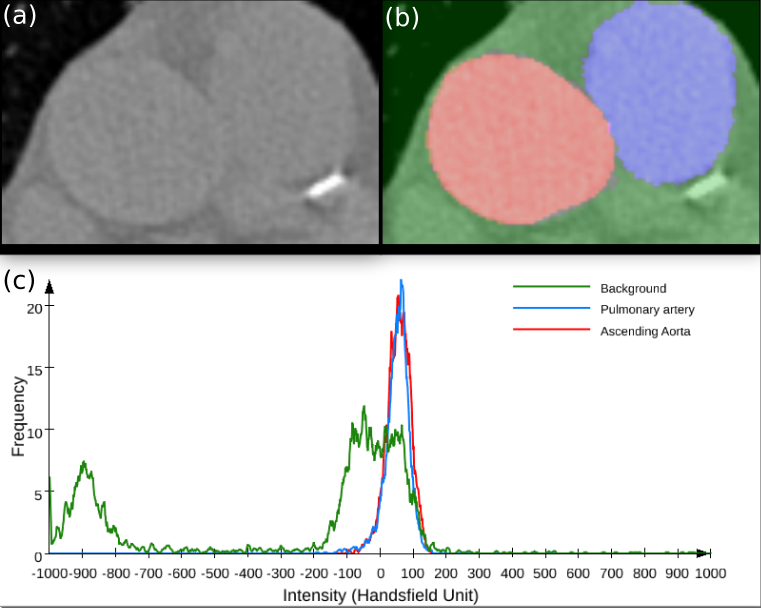
\includegraphics[width=0.60\textwidth]{Figures/vol13_intensityDistribution_2.png}
%    \resizebox{0.98\textwidth}{!}{{Figures/}{vol13_intensityDistribution_2.png}}
    \caption{(a) Axial plan of a non-contrast \gls{CT} at region of interest(ROI).(b) ROI overlaid with manual annotations of the aorta in red, pulmonary artery in blue and the background in green.(c) Intensity distribution of voxels in the aorta(red), pulmonary artery(blue), and background(blue) within ROI.}\label{fig: Intensity_Distribution}
\end{figure} 

Manual analysis of the vessels in cardiac CT requires prior experience and expertise to identify and locate geometrical structures. Since the aorta and pulmonary artery are large vessels that can be affected by pathology at multiple locations along all their length, the entire vessel should be imaged and measured. The most accurate quantification of the aorta and pulmonary artery dimensions is obtained by a full 3D analysis. Manual analysis require drawing the vessel contours in a large number of reformatted slices perpendicular to the vessel axis. This is a very labor-intensive and time-consuming process and subject to intra- and inter-observer variability. Manual measurement introduces other technical problems such as differences in slice thickness, image windowing/presentation, measurement location, and determining vessel edges/lengths. Furthermore, human workload is a limiting factor when performing quantitative measurements in large-scale imaging studies and in clinical practice. Automated analysis are therefore desirable and could add significant value in standardization and reproducibility of vessel segmentation and subsequent diameter analysis.

Automatic segmentation of the aorta and pulmonary artery in non-contrast non-\gls{ECG}-gated \gls{CT} scans is a challenging task in many aspects. There are three main challenges. The first challenge is the unclear vessel boundaries due to the lack of contrast between blood pool regions, muscle walls and fat (see Figure \cref{fig:Intensity_Distribution} ).  Second challenge is the proximity of the aorta and pulmonary artery to eachother and to other structures with similar intensity values such as heart. Figure \cref{fig:Intensity_Distribution} illustrates the intensity similarity between vascular area and the surrounding voxels in the region of interest (ROI) which is a region close to the heart chamber. The obvious overlap between the background and voxels within the aorta and pulmonary artery shows the difficulty in segmenting vascular area from the background. Furthermore, the similarity in the aorta and pulmonary artery intensity distribution and the unclear boundary between them (Figure \cref{fig:Intensity_Distribution}(a)), demonstrates the difficulty in detecting the correct border of the vessels. Additional challenges in non-ECG-gated \gls{CT} scan as is commonly used in lung screening, are motion artefacts caused by motion of the heart during the cardiac cycle and unclear vessel boundaries at the regions close to the heart where even manual measurements is difficult for experienced radiologists.



%Due to the complex 3D anatomy of the aorta and Pulmonary artery trunk 
%
%
%Due to
%the complex 3D anatomy of the aorta, it has been postulated that axial measurements
%of aortic diameters are not representative of real dimensions of the vessel

Diameter measurement for the aorta and pulmonary artery are not clinically standardized. Most clinicians measure the greatest diameter of the pulmonary artery on the axial scans, which can vary depending on the slice orientation with respect to the patient. Also due to the complexity of aortic anatomy specially at the aortic root, axial measurements of aortic diameters are not representative of real dimensions of the vessel. Therefore, automatic and precise diameter measuring techniques on plans perpendicular to the longitudinal axis, namely the vessel centerline, in standard landmark levels are more reliable and reproducible.

%Automatic diameter measurement is also difficult since there is no clinically standardize ways for measuring the diameters of aorta and pulmonary artery.
%
%Measurement of MPA diameter is difficult to standard-
%ize clinically, as most clinicians just measure the greatest diameter on the axial scans, which can vary depending on the slice orientation with respect to the patient. We therefore chose perimeter as our estimator of cross-sectional diameter because it is more reproducible duringmanual measurement, and would be a good representation of average diameter
%
%
%yields additional challenges for imaging techniques such as the proximity to the heart and
%consequent transmitted movements and the more complex anatomy.
%
%Features such as density, geometry,
%topology and size of vessels could be analyzed in diseases that imply vasculature
%remodeling, making even possible the discovery of new specific biomarkers that
%remain hidden nowadays. 
%
%Therefore, precise, reliable
%and reproducible aortic diameter measurements based on imaging techniques are a
%fundamental prerequisite for a correct management of aortic pathologies.




%In image analysis the first step is detection and separation of the required artery. 
%The most accurate quantification of the aorta and pulmonary artery dimensions is obtained by a full 3D analysis. Manual analysis require drawing the vessel contours in a large number of reformatted slices perpendicular to the vessel axis. This is a very labor-intensive and time-consuming process and subject to intra- and inter-observer variability. Furthermore, human workload is a limiting factor when performing quantitative measurements in large-scale imaging studies and in clinical practice. Therefore, automated analysis for vessel segmentation and subsequent diameter analysis are desirable.



%
%
%This is true not only for the abdominal aorta but also for the thoracic aorta that yields
%additional challenges for imaging techniques such as the proximity to the heart and
%consequent transmitted movements and the more complex anatomy. Furthermore, the
%thoracic aorta is often involved in genetic diseases such as connective tissue diseases and
%in patients with bicuspid aortic valves
%   
%non contrast vs contrast enhanced ===>
%Separation of arteries and veins is even more difficult in this scenario comparing
%with images where contrast agents are injected to the patients and differentiation
%between arteries and veins can be aided if a proper trigger for acquisition is used.
%
%low dose ==> high noise levels
%
%Low-dose computed tomography (CT) imaging provides a method for obtaining accurate anatomical information without the full radiation exposure inherent in standard CT protocols, and is primarily used in lung cancer screening. Segmentation of the pulmonary arteries from low-dose chest CT images is a vital first step in improving computer-aided detection of frequently missed pulmonary nodules near major arterie
%
%However, low-dose CT images present an additional
%challenge to segmentation methods, as there is less information and more noise
%than in standard-dose CT images
%
%non ecg gated ==> motion artifacts
%As a rule, electrocardiogram (ECG) gating is not used for these types of studies, and therefore motion artefact will impact the ability to assess the coronary arteries.
%
%
%challenge complexity and approximidity to heart ==>
%additional challenges for imaging techniques such as the proximity to the heart and
%consequent transmitted movements and the more complex anatomy.
%
%
% 
%The only recommended screening test for lung cancer is low-dose computed tomography (also called a low-dose CT scan, or LDCT).
%           
%
%ct and low contrast is better due to low radiation and low explotier . regular ct is what we can use


%\section{Imaging processing}

%Features such as density, geometry,
%topology and size of vessels could be analyzed in diseases that imply vasculature
%remodeling, making even possible the discovery of new specific biomarkers that
%remain hidden nowadays. 
%
%
% Nevertheless, the variety of different
%possible methods to measure aortic diameters hasn’t been completely addressed in
%guidelines and there is still no precise consensus on which technique should be employed.
%Since the aorta is a single organ that can be affected by pathology at multiple locations
%along all its length, the entire vessel should be imaged and measured.
%
%
%Although diastole
%is generally preferred because of better reproducibility and image quality, there is still no
%general consensus about which one should be employed [6].This is particularly relevant
%for the proximal portions of the aorta where, due to transmitted pulsation movements,
%aortic diameters change significantly during the cardiac cycle. Another unsolved issue is
%whether the aortic wall thickness should be included in aortic diameter measurements.
%At present, in clinical practise there is often a difference between imaging techniques
%considering that measurements are performed leading-edge to leading-edge on
%echocardiographic images (2DE) and inner-edge to inner-edge on CT and MRI images
%


%Segmentation of the pulmonary arteries also provides a first step toward obtaining highly accurate measurements of vessel radii. Patients with pulmonary
%arterial hypertension (PAH) have been shown to present with enlarged pulmonary
%arteries, as measured by manual observation of CT images [22, 17]. These enlarged
%vessels are at increased risk for fatal dissection and require immediate surgical intervention where possible. Automated segmentation and measurement methods
%have the potential to better quantify vessel enlargement in patients with PAH,
%providing an earlier and non-invasive means of diagnosis [14].



%\section{Vessel Segmentation}

presented methods in the past and the gap I tried to fill in my thess, then the latest improvements specially with deep learning



\section{Segmentation Methods} \label{sec:Segmentation}

Automatic and semi-automatic segmentation of the aorta and pulmonary artery have been the topic of studies in MRI \cite{berhane2020fully} and \gls{CTA} \cite{ecabert2011segmentation, biesdorf2012segmentation, entezari2013analysis, gao2016automatic, gao2017quantification, cao2019fully, linguraru2010segmentation, moses2016automatic, roman20183d,baskaran2020automatic}. Most fo these studies obtain reasonable segmentations due to the high contrast and resolution between the vessels, fat, and muscles. However, these methods do not translate well to non-contrast \gls{CT} scans where the vessel boundaries are not well defined in many places. Furthermore, the high noise level in low-dose scans and motion artifacts in non-\gls{ECG}-gated \gls{CT} scans result in even more unclear vessel boundaries which intensify the difficulty of the automatic segmentation. Therefore, relatively fewer studies can be found on non-contrast \gls{CT} scans, on the segmentation of the aorta \cite{ isgum2009multi,avila2013segmentation, dasgupta2017morphological, tahoces2019automatic, kitasaka2002automated, feuerstein2009automated, xie2014automated, kurugol2015automated,  noothout2018automatic,tahoces2019automatic,trullo2017joint, he2020multi} and pulmonary artery containing the pulmonary trunk, left, and right pulmonary arteries \cite{feuerstein2010adaptive, xie2015automated,bruns2019cnn}.

The existing segmentation methods, can be classified into three main groups: basic image processing methods \cite{isgum2009multi, avila2013segmentation, dasgupta2017morphological,tahoces2019automatic, }, embedding shape prior methods\cite{feuerstein2009automated, feuerstein2010adaptive, kitasaka2002automated, xie2014automated, xie2015automated, kurugol2015automated}, and deep learning methods\cite{trullo2017joint, he2020multi, noothout2018automatic, bruns2019cnn}.

Basic image processing methods includes the methods of multi-atlas models \cite{isgum2009multi}, active \cite{dasgupta2017morphological} and statistical shape models. These methods mainly are time consuming or require human interaction either for seed point placement or for parameter adjustment. 


Embedding shape priors methods with the use of shape priors generally have a better performance. These techniques, such as level set methods \cite{kurugol2015automated}, restrict the final segmentation to a pre-defined shape and are able to obtain impressive results. A limitation of level set methods is the existence of high-order functions and the resulting complex optimization problems which makes them slow. 



%Taeprasartsit et al.\cite{Taeprasartsit2007,Taeprasartsit2011}, employed model fitting to an Euclidean distance transformation based likelihood image to extract the center of the aorta and pulmonary artery. They applied region growing to segment the vessels.
%Feuerstein et al.\cite{Feuerstein2009,Feuerstein2010} proposed a Hough transform based adaptive model where they used Hough and Euclidean distance transforms and probability weighting to segment the aorta and the pulmonary arteries.
%Isgum et al.\cite{Isgum2009}, proposed a multi-atlas registration method for the aorta segmentation. In their method atlases where combined locally based on the registration success of each atlas.
%Kurkure et al.\cite{Kurkure2008} used fast marching-based minimal path extraction algorithm to extract the centerline and then used dynamic programming to detect the aortic boundary contour.
%All mentioned methods require human interaction either for seed point placement or for parameter adjustment. 
%
%Xie et al.\cite{Xie2014, Yiting2015} employed
%a cylinder matching method to extract the centerline of the aorta and pulmonary arteries. To segment the vessels they used geometric constraints obtained from other adjacent organs from a pre-computed anatomy label map. Although the obtained results are good, an anatomy map is not always available.
%Level sets \cite{Kurugol2015a} and active contours\cite{Dasgupta2017} are succesful methods for vessel segmentation.
%Kurugol et al.\cite{Kurugol2015a}, employed Hough transforms on reformatted oblique slices to have an initial rough boundary of the aorta. Thereafter they refined the boundaries by a 3D level-set segmentation.
%86\% of the used data where contract enhanced CT.
%Tahoces et al.\cite{Tahoces2019} used an ellipse estimation algorithm and an energy-based optimization technique to automatically track the centerline and the cross sections of the aorta. Although, they achieved a good segmentation results, the resulted volumes from cross sections are not smooth. 
%
%Deep learning is being used widely in medical image segmentation in the recent years\cite{Lopez-LinaresRoman2018,Trullo2017,Noothout2018} however, only few are presented on non-contrast CT\cite{Trullo2017,Noothout2018}. Trullo et al.\cite{Trullo2017} proposed a two collaborative SharpMask architecture to jointly segment esophagus, heart, aorta and trachea. They extract low-level and deep high-level features and the special relation between the organs by the use of Conditional Random Fields in the first deep architecture and then refined the segmented organs in the second deep architecture. Noothout
%et al.\cite{Noothout2018}, employed a dilated CNN to segment the aorta on ECG gated scans. The above mentioned deep learning methods have a low accuracy and need a more complex network to segment the aorta and pulmonary artery.
%
%
%Graph-cut based methods have been used in medical image segmentation\cite{Chen2018,Deng2018,Jimenez-Carretero2019,Arias-Lorza2015} and have obtained promising results in many tasks. 
%Deng et al.\cite{Deng2018} proposed a graph-cut method using random forest based discriminative features on non-contract CT for aorta segmentation. They achieved a high segmentation performance in the abdominal aorta, however, they have not applied their method to the thoracic aorta which is more challenging to segment due to unclear vessel boundaries especially in the heart chamber region and the shape variation in aortic arch.
%Jimenez-Carretero et al.\cite{Jimenez-Carretero2019} use local information and a specifically designed graph-cut methodology to segment the pulmonary artery vein in non-contract CT scans,however, they have not extracted the main pulmonary branches.
%
%Arias et. al.\cite{Arias-Lorza2015} proposed a semi-automatic 3D optimal surface graph-cut algorithm to segment the carotid artery wall in MRI scans. They define the graph columns based on flow lines traced from a coarse initial segmentation where the non-intersecting flow lines guarantee non self-intersecting surfaces in high curvature area. 
%%There method guarantees global minimization of a cost function, ensuring smooth surfaces and topological constraints between surfaces.%
%Optimal surface graph cut methods have the possibility to enforce topology constraints and to incorporate an initialization volume in the graph structure.
%
%In this paper we present an extension of our previous work\cite{SedghiGamechi2018a} which uses an optimal surface graph cut based method to segment the aorta and pulmonary arteries on non-contract CT scans.
%In our previous work\cite{SedghiGamechi2018a} human interaction was required for seed point placement. In this paper we present a full automatic method which the seed points and a landmark for the pulmonary artery bifurcation level are extracted by applying a multi-atlas registration method. The method employs multiscale medialness filters and lumen intensity similarity followed by minimum cost path tracking to extract the centerlines and radius estimation of the aorta and pulmonary arteries. Thereafter, centerlines are refined by re-computing the minimum cost path after curved multi-planar reformatting (CMPR) and are dilated non-uniformly based on the vessel radius estimation. Subsequently for each vessel a graph is constructed with non-intersecting columns based on flow lines and a graph cut is applied to find the optimal surface.
%From the 3D derived vessel segmentation we automatically measure the vessel diameters and the PA:AA ratio in the level of the pulmonary artery bifurcation both in 2D axial slices and in 3D volumes around the level of pulmonary artery bifurcation.
%The key contributions of the presented method are (a) full automatic aorta and pulmonary artery segmentation method. (b) 3D volumetric measurements of PA and AA diameters and the PA:AA ratio.
%
%use this text for CT \cite{McCollough2009}
%Risk of ionizing radiation exposure from CT scans  \cite{Kumar2016}
%\gls{COPD} apportunity to discover in lung CT scans \cite{Tang2020}
%
%

Another approach is to use graph cut methods with shape priors. Graph cuts can achieve a global optimum with low processing times and it is possible to incorporate shape constraints in the graph structure. Graph cut methods have been applied to different imaging modalities for artery segmentation \cite{deng2018graph, arias2015carotid} and have obtained promising results in many tasks. Deng et al. \cite{deng2018graph} proposed a graph-cut method using random forest based discriminative features on non-contrast \gls{CT} for aorta segmentation. They achieved a high segmentation performance in the abdominal aorta, however, they have not applied their method to the theoratic aorta and pulmonary artery which are more challenging to segment. In this thesis we will present an optimal surface graph cut approach similar to Petersen et al. \cite{petersen2014optimal} for pulmonary artery and aorta segmentation. This method incorporates a shape prior via constructing the graph based on flow lines traced from an initial, smoothed segmentation. The non-intersecting flow lines guarantee non-self-intersecting surfaces and make it possible to segment high curvature areas such as the bifurcation of the pulmonary artery and the aortic arch while guaranteeing a shape that is similar to the initialization shape.


Besides the high performing graph-cut techniques for medical image segmentation, deep learning techniques are being used widely in the recent years \cite{roman20183d, trullo2017joint, noothout2018automatic, bruns2019cnn, chen2020deep,dou20173d, fantazzini20203d}. Deep learning based algorithms have the advantage of directly learning from data in an end-to-end fashion using a general-purpose learning procedure. With the increasing amount of data to learn from, deep learning based algorithms have gradually outperformed previous methods. Chen et al \cite{chen2020deep} have compared current techniques for segmenting cardiovascular structures in different imaging modalities where among the big diversity of deep learning techniques, deep \gls{CNN}s have achieved remarkable performance and shown a great success in many segmentation tasks. However, there are still few studies performed on aorta segmentation on non-contrast \gls{CT} scans \cite{trullo2017joint, noothout2018automatic, bruns2019cnn} and to the best of our knowledge there are no deep learning based algorithms presented for the segmentation of the pulmonary artery trunk and its major branches on non-contrast \gls{CT} scans. 


 CNNs are supervised neural networks that have the ability to learn highly discriminative spatial and spectral features resulting in relatively smooth segmentation. Whereas the lack of directly modeling iteractions between predictions and not using context information result in poorly segmented boundaries and edge-precise segmentation remains a challenging issue. To address this challenge, in this thesis we will present an end-to-end training method based on the combination of a \gls{CNN} (such as U-net) with a \gls{CRF}. CRFs are probabilistic graphical models that model the correlations and dependencies among the voxels being predicted. Although, it is common to combine \gls{CNN} with a \gls{CRF} to refine the voxel-level predictions made by \gls{CNN}, \gls{CRF} was often used as a post-processing technique by encouraging spatial coherence. However, due to the intensity similarity between vessels and surrounding structures, intensity-based information alone provides a low-quality, feature space for the CRF. Therefore, in this thesis the presented end-to-end method named Posterior-CRF, allows the CRF to use features learned by a \gls{CNN}, optimizing the \gls{CRF} and \gls{CNN} parameters concurrently. In this thesis the proposed Posterior-CRF is applied for jointly segmenting the aorta and pulmonary artery on non-contrast \gls{CT} scans.




%To this end, combining probabilistic graphical models such as Markov Random Field (MRF) and Conditional Random Field (CRF) with CNN brings signifi- cant improvements by explicitly modelling the dependencies between regions
%
%CNN Positive:
%great model capacity and the ability to learn highly discriminative features for the task at hand. 
%
% 
%The convolutional neural network-based (CNN-based) feature encoders enable spatial and spectral feature extractions and output representative feature vectors, which can be used as the backbone for dense classification tasks.Learnable parameters [16–21] or network structures [22,23] push models to fit the feature space and reach the accurate pixel-wise classification results
%
%CNN negitive:
%
%they lack the capability to utilize context information and cannot model interactions between predictions directly. Due to the discrete cost functions and the inflation of receptive fields in CNN-based feature extractors, neural image segmentation is restricted to coarse pixel-level classification
%
%Conditional Random Fields (CRFs) are probabilistic graphical models which model the correlations between the voxels being predicted. 
%where they result in obtaining smooth edges
%
%
%
%The convolutional neural network-based (CNN-based) feature encoders enable spatial
%and spectral feature extractions and output representative feature vectors, which can be used as the
%backbone for dense classification tasks.Learnable parameters [16–21] or network structures [22,23]
%push models to fit the feature space and reach the accurate pixel-wise classification results. Due to the discrete cost functions and the inflation of receptive fields in CNN-based feature extractors, neural image segmentation is restricted to coarse pixel-level classification
%
%
%Because CNN can effectively discover spatial structures among the neighboring patches of the input data, the resulting classification maps generally appear smoother in spite of not modeling the neighborhood dependencies directly. However, the possibility of reaching local minima during training of CNN and the presence of noise in the input images may create holes or isolated regions in the classification map. Compared with other machine learning methods, CNN is generally limited by the absence of shape and edge constraints. As a result, the final segmentation appears rough on edges. In these circumstances, a further step of segmentation produce much refined output. To this end, combining probabilistic graphical models such as Markov Random Field (MRF) and
%Conditional Random Field (CRF) with CNN brings significant improvements by explicitly modelling the dependencies
%between regions. CRFs have been used to model important geometric characteristics such as shape, region connectivity, contextual information between regions and so on. For these reasons, there has been a recent trend on exploring the integration of CNN and CRF methods
%
%Despite many efforts had been taken on the improvement, the result was still unsatisfactory, especially, on the boundary ofthe object. 
%
%
%whereas edge-precise segmentation remains a challenging issue
%
%*******

%Due to the intensity similarity between the aorta, pulmonary artery and the surrounding structures in non-contrast CT scans, vessel segmentation is a challenging task even for CNNs. In CNNs the presence of convolutional filters with large receptive fields and the lack of smoothness constraints that encourage label agreement between similar voxels, and spatial and appearance consistency of the labelling output, can result in coarse segmentations \cite{long2015fully, zheng2015conditional}.




\section{Outline of this thesis} \label{sec:Goals}
Given the segmentation challenges and the described available literature, the focus of this thesis is on development and validation of techniques that aim to automatize the segmentation of the aorta and pulmonary artery, and subsequently diameter measurements on non-ECG-gated, non-contrast \gls{CT} scans. The outline and the structure of this thesis is as follows:

\begin{description}
    \item[\cref{chap:Aorta_Segmentation}] presents a full automatic method based on optimal surface graph-cuts for the segmentation of the aorta on non-ECG-gated, non-contrast CT from the Danish lung cancer screening dataset. Thereafter ,from the extracted 3D aorta segmentation, the diameter of the ascending and descending aorta are calculated at cross-sectional slices perpendicular to the extracted centerline, at multiple, fixed levels relative to the pulmonary artery bifurcation level.    

    \item[\cref{chap:Pulmonary_Segmentation}] presents a 3D full automatic segmentation method for segmenting the pulmonary artery as well as the aorta with a similar method as presented in \cref{chap:Aorta_Segmentation}. The method extracts a landmark for the level of the pulmonary artery bifurcation. With the 3D volumetric average diameter measurement technique presented in this chapter, the ratio of the diameter of the pulmonary artery to the diameter of the ascending at the level of the pulmonary artery bifurcation is automatically extracted and validated.

    \item[\cref{chap:Growth}] makes use of the method presented in \cref{chap:Aorta_Segmentation} for extracting aortic diameters for the investigation of the growth of the theoretic aorta. This study presents longitudinal data on sex-specific growth of the ascending and descending aorta in a large population of current or former smokers. 
    
    
    \item[\cref{chap:Posterier_CRF}] presents an deep learning based algorithm where an end-to-end segmentation method called Posterior-CRF uses CNN-learned features in a CRF. This method is validated on multiple modalities and medial image segmentation tasks. The aorta and pulmonary artery are segmented in non-contrast CT, white matter hyperintensities and ischemic stroke lesion are segmented in multi-modal MRI. 
    
    \item[\cref{chap:Discussion}] provides a general discussion of the results and achievements of this thesis and presents possible future research directions.

\end{description}

